\documentclass{standalone}
\usepackage{tikz}
\usetikzlibrary{decorations.pathreplacing}
\usepackage{amsfonts}


\begin{document}
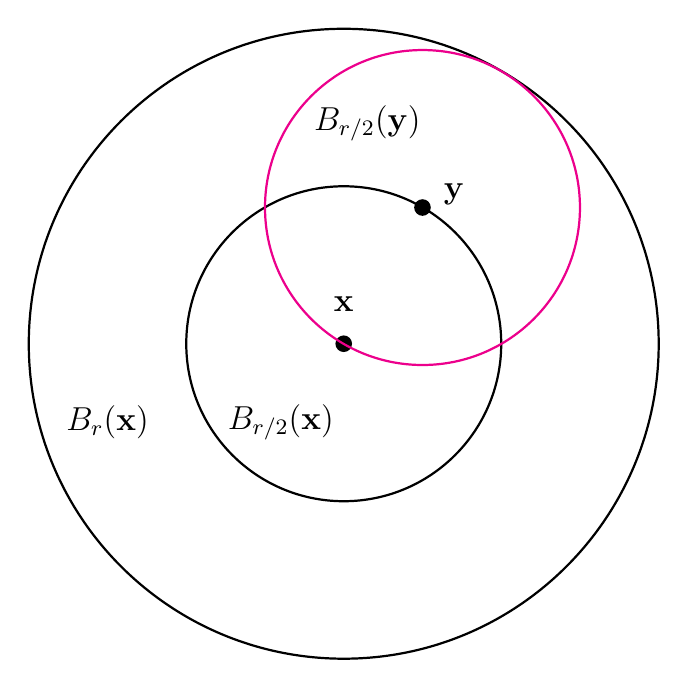
\begin{tikzpicture}
  % Draw the ellipse A
  \draw[thick] (0,0) circle (4cm);
  
  \draw[thick] (0,0) circle (2cm);

  \node at (-3,-1) {\large$B_r(\mathbf{x})$};
  
  \node at (-0.8,-1) {\large$B_{r/2}(\mathbf{x})$};
  
  \fill (0,0) circle (3pt);
  \node at (0,0.5) {\large$\mathbf{x}$};
  
  % Center of the ball x
  \fill (1,1.73) circle (3pt);
  \node at (1.4,1.9) {\large$\mathbf{y}$};
  
  % Draw the ball B_r(x)
  \draw[magenta, thick] (1,1.73) circle (2cm);
  \node at (0.3,2.8) {\large$B_{r/2}(\mathbf{y})$};
  

  
  
\end{tikzpicture}
\end{document}
